\section{Thermal shield vibrations}\label{sec:5:thermal-vibrations}
A spherical plate that is fixed at the edge can vibrate in different vibrational modes labeled by the indices $(k,l)$ where $k \in [1,\infty)$ and $l \in [0, \infty)$.
The exact vibrational frequency and the mode shape can only be given in terms of the Bessel functions. In fact, one of the first occurrences of these functions can be traced back to Euler trying to solve the very similar problem of a vibrating perfectly flexible membrane \cite{Dutka_1995}.
In general, the vibrations of a plate with thickness $d$ can be described by the differential equation \cite[p. 490]{Rao_2019}
\begin{equation}
  D \nabla^2\nabla^2 u = -\rho d \ddot{u}
\end{equation} 
where $D$ is given by material properties like Youngs module $E$ and the poisson number $\nu$ as
\begin{equation}
  D = \frac{d^3 E}{12(1-\nu^2)} .
\end{equation}
The general solution of this differential equation can be written in terms of the Bessel functions as (derived in Ref. \cite[p. 490-495]{Rao_2019}) 
\begin{equation}
  u_{kl}(r, \theta, t) = z\left[J_l(\beta_k r) - \frac{J_l(\beta_k r_s)}{I_l(\beta_k r_s)}I_l(\beta_k r)\right]\cos(l\theta+\phi_1)\sin(\omega_{kl}t+\phi_2)
\end{equation}
with
\begin{equation}
  \beta_k = \frac{\tilde{r}_k}{r_s} \quad \text{and} \quad \omega_{kl} = \frac{\tilde{r}_k^2}{r_s^2}\sqrt{\frac{D}{\rho d}} = \tilde{r}_k^2\frac{d}{r_s^2}\sqrt{\frac{E}{12\rho(1-\nu^2)}} ,
\end{equation}
where $\tilde{r}_k$ is the $k$-th solution of the equation
\begin{equation}
  J_l(\tilde{r}_k)I_{l+1}(\tilde{r}_k)+I_l(\tilde{r}_k)J_{l+1}(\tilde{r}_k) = 0 .
\end{equation}
The phases $\phi_1$ and $\phi_2$ can be determined by initial conditions and refer to the rotation of the plate as well as temporal offsets. The first few modes are shown in \cref{fig:5:vibrational-modes}.
\begin{figure}[!ht]
  \centering
  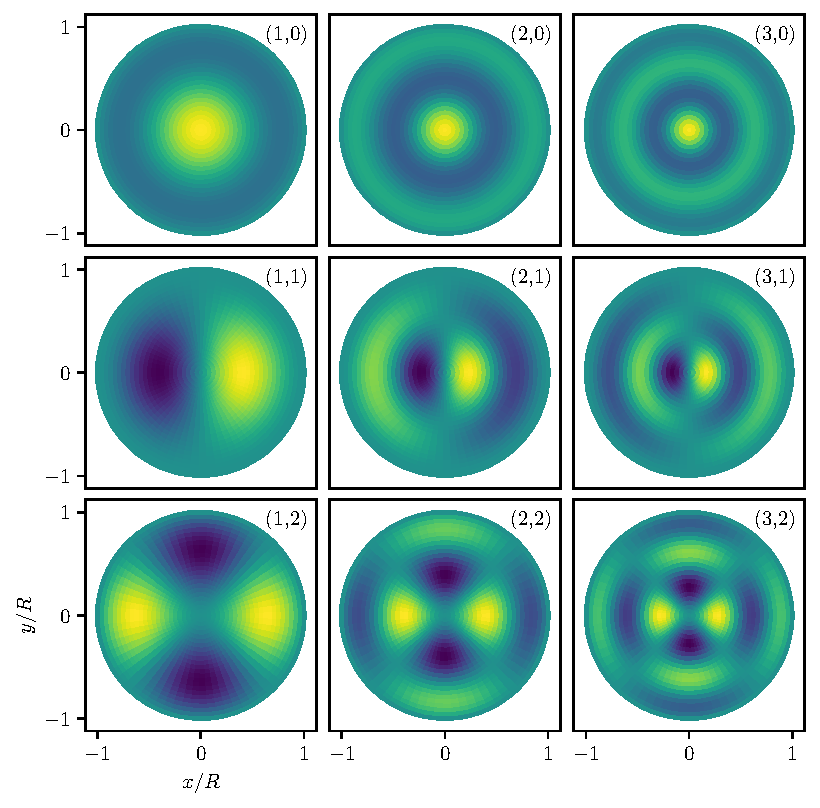
\includegraphics[width=\textwidth]{./../figures/vibrations/vibrational-modes.pdf}
  \caption{Normalized shape of the vibrational modes $(k,l)$ of a vibrating spherical plate fixed at the edge with $R/d = 1000$.}
  \label{fig:5:vibrational-modes}
\end{figure}
In general, every possible vibration of the plates can be expressed as a sum of these default modes $u_{kl}$. The amplitude $z$ of the vibrations are determined by the thermal temperature and can be estimated by treating the amplitude of each vibration as a quantum harmonic oscillator with frequency $\omega_{kl}$.
The expectation value of the amplitude $\avg{\op{z}}$ is obviously zero and the variance $(\Delta \op{z})^2 = \avg{\op{z}^2} - \avg{\op{z}}^2$ at temperature $T$ is given by
\begin{equation}\label{eq:5:amplitude-variance}
  (\Delta \op{z}_{kl})^2_T = \frac{\hbar}{2\tilde{m}\omega_{kl}}\coth(\frac{\hbar \omega_{kl}}{2k_BT}) \approx \frac{k_B T}{\tilde{m}\omega_{kl}^2}
\end{equation}
A derivation of this is given in appendix \ref{apx:thermal-harmonic-oscillator}.
In the last step $\hbar\omega \ll k_B T$ was used. $\tilde{m}$ is the \textit{effective mass} of the mode in which the precise shape is considered. A intuitive estimation for this mass can be given by the average of the mode 
\begin{equation}\label{eq:5:effective-mass}
  \tilde{m} = m\frac{1}{\pi r_s^2}\int_0^{r_s} \dd r \int_0^{2\pi} r\dd\theta \, u_{kl}(r, \theta, t) .
\end{equation}
with $m=\rho \pi r_s^2 d$ being the total mass of the shield.


\subsection{Occupation of the vibrational modes}



\begin{equation}
  \op{H} = \hbar \omega \left(\op{a}^\dagger\op{a} + \frac{1}{2}\right) + \tilde{g}_A(\op{z}) \ketbra{\psi_A} + \tilde{g}_B(\op{z}) \ketbra{\psi_B}
\end{equation}

Solution:
\begin{equation}
  \rho(t) = \frac{1}{2}\begin{pmatrix}
    1 & e^{-i\varphi(t)}e^{-\gamma(t)}\\
    e^{i\varphi(t)}e^{-\gamma(t)} & 1
  \end{pmatrix}
\end{equation}
with the phase
\begin{equation}
  \varphi(t) = \frac{1}{\hbar^2\omega^2} \left(\sin(\omega t) - \omega t\right) \left(g_A^2 - g_B^2\right)
\end{equation}
and the decoherence term
\begin{equation}
  \gamma(t) = \frac{4(g_A - g_B)^2}{\hbar^2 \omega^2} \sin^2\left(\frac{\omega t}{2}\right) \left[\bar{n} + \frac{1}{2}\right]
\end{equation}

\begin{figure}[!htbp]
  \centering
  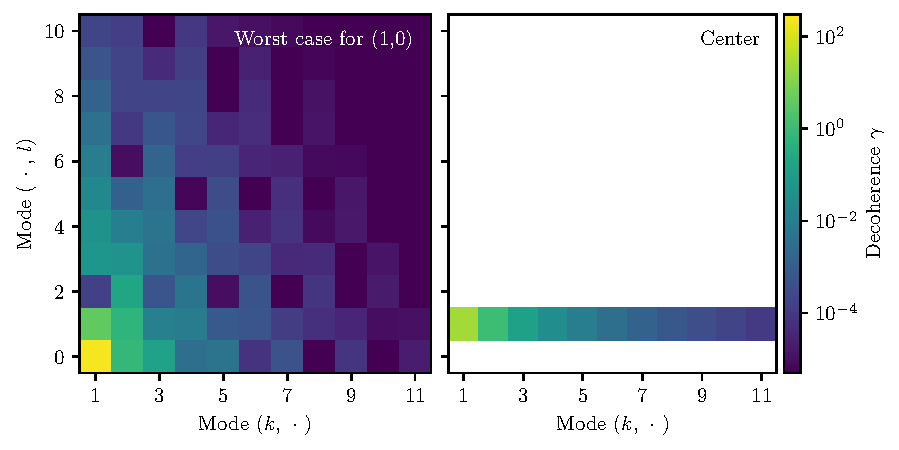
\includegraphics[width=\textwidth]{./../figures/vibrations/decoherence-analytical.pdf}
  \caption{Maximum decoherence $\gamma$ at $4\si{K}$ for all modes if the cat-state is placed \textbf{left:} at the point with maximum gradient of the mode $(1,0)$ and \textbf{right:} in the center of the plate. It becomes evident, that only a few low modes play an actual role for the total dephasing.}
  \label{fig:5:}
\end{figure}


\begin{figure}[!htbp]
  \centering
  \def\svgwidth{\textwidth}
  \input{./../figures/plate-vibration.pdf_tex}
  \caption{For a large shield, vibrations can be interpreted locally as if one mass was a distance $\Delta L$ further away from a shield and the other one $\Delta L$ closer and as if both masses would be rotated by an angle $\Delta \theta$.}
\end{figure}